%%=============================================================================
%% Resultaten
%%=========================================================================
\chapter{Resultaten}
\label{ch:resultaten}

\section{Resultaten vragenlijst}
\label{sec:Resultaten vragenlijst}
In totaal zijn er 548 online deelnames geregistreerd voor de vragenlijst. In de onderstaande tabel worden de antwoorden overlopen. In de 2de kolom is de som van de antwoorden terug te vinden en de laatste kolom toont het procent van het antwoord op de vraag ten opzichte van het totaal. De analyse is gemaakt in Rstudio, het script is terug te vinden in de bijlages.
\begin{table}[h!]
\begin{center}
\begin{tabular}{ |p{10cm}|p{2cm}|p{2cm}| }
 \hline
 \multicolumn{3}{|c|}{Algemene gegevens} \\
 \hline
 \textbf{Geslacht} & \textbf{N = 548} &\textbf{Procent}\\ 
 \hline
 Vrouwen   & 250    &45.6\%   \\
 Mannen &   298  &54.4\%   \\
 \hline
 \textbf{Leeftijd deelnemers in 2 klasses} & \textbf{N = 548} &\textbf{Procent}\\ 
 \hline
 leeftijd <= 25   & 300    &54.7\%   \\
 leeftijd > 25 &   248  &45.3\%   \\
 \hline
  \textbf{Hoe vaak sport u per week? } & \textbf{N = 548} &\textbf{Procent}\\ 
 \hline
 minder dan 1 keer   & 90    &16.4\%   \\
 1 keer &   66  &12\%   \\
 2 keer &   74  &13.6\%   \\
meer dan 2 keer &   318 &58\%   \\
 \hline
     \textbf{Heeft u al een mobile coaching applicatie gebruikt?} & \textbf{N = 548} &\textbf{Procent}\\ 
 \hline
Ja   & 292    &53.3\%   \\
Nee &   256  &46.7\%   \\
  \hline
\end{tabular}
\end{center}
\end{table}

\vspace{1cm}
\begin{table}[h!]
\begin{center}
\begin{tabular}{ |p{10cm}|p{2cm}|p{2cm}| }
 \hline
    \textbf{Welk besturingssysteem heeft uw smartphone?} & \textbf{N = 548} &\textbf{Procent}\\ 
 \hline
IOS   & 206    &37.6\%   \\
Android &   330  &60.2\%   \\
overig &   12  &2.2\%   \\
 \hline
 \multicolumn{3}{|c|}{Functionele requirements} \\
 \hline
     \textbf{Vindt u het belangrijk om de applicatie met een smartwatch of dergelijke te connecteren?} & \textbf{N = 548} &\textbf{Procent}\\ 
 \hline
Ja   & 306    &55.8\%   \\
Nee &   242  &44.2\%   \\
 \hline
     \textbf{Is het belangrijk dat u de applicatie kan koppelen aan social media? (Facebook,Twitter,...)} & \textbf{N = 548} &\textbf{Procent}\\ 
 \hline
Ja   & 110    &20\%   \\
Nee &   438  &80\%   \\
 \hline
      \textbf{Vindt u het belangrijk dat een applicatie gebruik maakt van uw geolocatie (GPS)? bv. om uw traject te zien} & \textbf{N = 548} &\textbf{Procent}\\ 
 \hline
Ja   & 362    &66\%   \\
Nee &   186  &34\%   \\
 \hline
       \textbf{Ik vind extra uitleg of filmpjes bij oefeningen...} & \textbf{N = 548} &\textbf{Procent}\\ 
 \hline
Absoluut nodig   & 82    &15\%   \\
Soms handig &   414  &75.5\%   \\
Overbodig &   52  &9.5\%   \\
  \hline
 \multicolumn{3}{|c|}{Niet-functionele Requirements} \\
 \hline
        \textbf{Bent u bereid te betalen voor een applicatie?} & \textbf{N = 548} &\textbf{Procent}\\ 
 \hline
Ja   & 150    &27.4\%   \\
Nee &   398  &72.6\%   \\
 \hline
         \textbf{Hoe belangrijk vindt u het uitzicht en gebruiksgemak van een applicatie?} & \textbf{N = 548} &\textbf{Procent}\\ 
 \hline
Belangrijk   & 386    &70.4\%   \\
Niet bijzonder & 60   &11\%   \\
Ik kijk enkel naar de functies binnen de applicatie &   102  &18.6\%   \\
 \hline
          \textbf{Wat is uw hoofddoel bij het gebruik van een Mobile Coaching applicatie?} & \textbf{N = 548} &\textbf{Procent}\\ 
 \hline
Spieropbouw  & 180    &32.8\%   \\
Afvallen & 130   &25.2\%   \\
Fit blijven &   230  &42\%   \\
  \hline
 \multicolumn{3}{|c|}{Gebruikerstype} \\
 \hline
         \textbf{Welk type applicatie past best bij u?} & \textbf{N = 548} &\textbf{Procent}\\ 
 \hline
 Enkel voedingsschema & 134    &24.5\%   \\
Enkel trainingsschema & 216  &39.4\%   \\
Mobile Coach &   198  &36.1\%   \\
  \hline
\end{tabular}
\end{center}
  \caption{Resultaten online vragenlijst}
\label{table:1}
\end{table}
\newpage
Uit de vragenlijst blijkt dat er iets meer mannen dan vrouwen hebben deelgenomen. 318 deelnemers gaan meer dan 2 keer per week sporten. Ongeveer de helft heeft ooit al een mobile coaching applicatie gebruikt. Er kan ook afgeleid worden dat Android het meest gebruikte besturingssysteem is met 60,2\% in dit onderzoek. Gevolgd door IOS met 37,6\%. 
Volgende requirements vallen op uit cijfers van dit onderzoek. Algemeen kan er gezegd worden dat maar liefst 80\% geen belang hecht om de coaching applicatie te koppelen aan sociale media. Ongeveer 72\% van de deelnemers ziet het ook niet zitten om te betalen voor een mobile coaching applicatie. 70\% van de deelnemers vindt het uitzicht en gebruiksgemak van de applicatie belangrijk. 362 van de 548 deelnemers vindt het gebruik van geolocatie belangrijk. Het hoofddoel bij het gebruik van een mobile coaching applicatie is voor 42\% om fit te blijven, gevolgd door spieropbouw met 32,8\% en als laatste afvallen met 25,2\%.

Als de deelnemers moeten kiezen tussen de 3 gebruikerstypes dan wordt het vaakst voor “enkel trainingsschema” gekozen gevolgd door “mobile coaching” en als laatste  “enkel voedingsschema’s”. 


\subsection{Algemene gegevens  van mannen en vrouwen uit de bevraging}
\label{sec:Resultaten vragenlijst}
In dit onderdeel wordt er een algemeen beeld gevormd over de bevraagde groep. Er wordt meer inzicht gegeven over de antwoorden op de algemene vragen per geslacht. Dit kan vooral handig zijn als ontwikkelaar om een doelgroep uit te kiezen bij het ontwikkelen van een applicatie. In de tabel wordt het aandeel van de subgroep ten opzichte van het totaal aantal deelnemers geplaatst, in dit geval 548 personen. 
\begin{table}[h!]
\begin{center}
\begin{tabular}{ |p{10cm}|p{2cm}|p{2cm}| }
 \hline
 \textbf{Leeftijd deelnemers in 2 klasses} & \textbf{mannen} &\textbf{vrouwen}\\ 
 \hline
 leeftijd <= 25   & 36.9\%    &17.9\%   \\
 leeftijd > 25 &   17.5\%  &27.7\%   \\
 \hline
  \textbf{Hoe vaak sport u per week? } & \textbf{mannen} &\textbf{vrouwen}\\ 
 \hline
 minder dan 1 keer   & 6.6\%   & 9.9\%  \\
 1 keer &   6.6\%  & 5.5\%   \\
 2 keer &   4.6\%& 8.8\%   \\
meer dan 2 keer &  36.5\% & 21.5\%  \\
 \hline
   \textbf{Welk besturingssysteem heeft uw smartphone?}  & \textbf{mannen} &\textbf{vrouwen}\\ 
 \hline
IOS   & 19.3\%   &18.2\%   \\
Android &   35\%  &25.2\%   \\
Overig &   0\%  & 2.3\%  \\
 \hline
    \textbf{Heeft u al een mobile coaching applicatie gebruikt?}  & \textbf{mannen} &\textbf{vrouwen}\\ 
 \hline
Ja   & 29.8\%  &23.6\%   \\
Nee &   24.4\%  &22.2\%   \\
  \hline
\end{tabular}
\end{center}
\caption{Algemene gegevens  van mannen en vrouwen uit de bevraging}
\label{table:1}
\end{table}
\newpage
De algemene gegevens zijn ongeveer evenwichtig verdeeld tussen mannen en vrouwen. Er hebben wel bijna 37\% mannen jonger dan 26 jaar deelgenomen aan het onderzoek tegenover ongeveer 18\% vrouwen van dezelfde leeftijdscategorie. Zowel het grootste deel van de mannen ( 36.5\%) en vrouwen (21.5\%) gaat meer dan 2 keer per week sporten. Dit wil zeggen dat er heel wat mensen met ervaring hebben deelgenomen aan de enquête, wat een verrijking voor de antwoorden over de requirements kan betekenen. 


\subsection{Verschil in requirements tussen mannen en vrouwen}
\label{sec:Resultaten vragenlijst}
In onderstaande tabel worden de antwoorden van vrouwen en mannen tegenover elkaar geplaatst. Er wordt onderzocht als voor elk geslacht dezelfde functionaliteiten belangrijk zijn of als er significante verschillen zijn. De antwoorden die pro of contra zijn worden opgenomen in de tabel. In het geval dat er meer dan 2 antwoorden mogelijk waren op de vraag, zijn enkel de voorstanders en de tegenstanders opgenomen. De neutrale antwoorden zijn hier even uitgefilterd omdat we opzoek zijn naar duidelijke verschillen. De resultaten zijn terug te vinden in procent.
\begin{table}[h!]
\begin{center}
\begin{tabular}{ |p{2.5cm}|p{2.3cm}|p{2.3cm}||p{2.8cm}|p{2.9cm}| }
 \hline
     \textbf{Requirement} & \textbf{mannen pro} & \textbf{vrouwen pro} & \textbf{mannen contra} & \textbf{vrouwen contra } \\
 \hline
Connectie met smartwatch   & 24.1\%    &31.8\% & 30.3\%    &13.8\%   \\
 \hline
Sociale media koppelen  & 10.9\%    &9.2\% & 43.4\%    & 36.5\%   \\
 \hline
 Geolocatie  & 36.5\%    &29.6\% & 17.9\%    & 16.1\%   \\
 \hline
  Video bij oefening  & 9.5\%    &5.5\% & 7.3\%    & 2.2\%   \\
 \hline
   Betalende applicatie  & 17.9\%    &9.5\% & 36.5\%    &  36.1\%   \\
 \hline
   uitzicht en gebruiksgemak  & 41.6\%    &28.8\% & 8.4\%    &  10.2\%   \\
 \hline
\end{tabular}
\end{center}
  \caption{Verschil in requirements tussen mannen en vrouwen}
\label{table:1}
\end{table}
De meningen om externe apparaten te verbinden zoals smartwatches liggen verdeeld. Over het algemeen vinden vrouwen dit een grotere noodzaak dan mannen. Vrouwen en mannen hebben dezelfde mening over het koppelen van sociale media, maar ongeveer 10\% bij beide groepen vindt dat dit moet. Zowel een grote meerderheid van mannen en vrouwen vindt dat geolocatie een functie moet zijn. Over video’s bij oefeningen en betalende applicaties zijn vrouwen en mannen het opnieuw met elkaar eens want video’s vinden ze over het algemeen soms handig maar niet noodzakelijk en ze zijn allebei voorstanderd van gratis applicaties. Het valt wel op dat mannen met bijna 18\% en vrouwen slechts met 9\% kiezen om te betalen voor een applicatie. Mannen vinden het uitzicht en gebruiksgemak van een applicatie met 41.6\% toch belangrijker dan vrouwen met 28.8\%. Maar slechts een kleine groep van allebei vindt het uitzicht en gebruiksgemak niet onbelangrijk.
\subsection{Verschil in requirements tussen leeftijd}
\label{sec:Resultaten vragenlijst}
In dit onderzoek zijn de deelnemers opgesplitst in 2 groepen. De ene groep loopt tot en met een leeftijd van 25 en worden gezien als jongvolwassenen en jeugd. De andere groep vanaf 26 jaar wordt gezien als volwassenen. De keuze om te splitsen op deze leeftijd komt omdat de mediaan van de leeftijd op 25 jaar ligt. Er wordt dus gesplitst in de helft van alle leeftijden. Er wordt gekeken als de leeftijd afhangt van het antwoord die gegeven wordt op de vraag. De resultaten zijn terug te vinden in onderstaande tabel in procent. Opnieuw zijn de neutrale antwoorden er uitgefilterd om significante verschillen te zien tussen pro en contra. 
\begin{table}[h!]
\begin{center}
\begin{tabular}{ |p{2.5cm}|p{2.3cm}|p{2.3cm}||p{2.8cm}|p{2.9cm}| }
 \hline
     \textbf{Requirement} & \textbf{ =< 25 pro} & \textbf{> 26 pro} & \textbf{=< 25 contra} & \textbf{> 26 contra } \\
 \hline
Connectie met smartwatch   &24.4\%    &31.8\% & 30.2\%    &13.6\%   \\
 \hline
Sociale media koppelen  & 8\%    &12\% & 46.7\%    & 33.3\%   \\
 \hline
 Geolocatie  & 37.6\%    &28.4\% & 17.2\%    & 16.8\%   \\
 \hline
  Video bij oefening  & 9.9\%    &5.1\% & 6.9\%    & 2.6\%   \\
 \hline
   Betalende applicatie  & 14.2\%    &13.1\% &41.5\%    &  31.2\%   \\
 \hline
   uitzicht en gebruiksgemak  & 41.6\%    &28.8\% & 8.8\%    &  9.8\%   \\
 \hline
\end{tabular}
\end{center}
  \caption{Verschil in requirements tussen leeftijd}
\label{table:1}
\end{table}

Opnieuw liggen de meningen over de connectie met externe apparaten verspreid. De volwassengeneratie vindt deze functionaliteit net iets belangrijker dan de jongvolwassenen. Het koppelen van sociale media is voor beide groepen geen belangrijke functie. De jongvolwassenen vinden voor 37.6\% dat geolocatie een must is en de volwassenen vinden dit voor 28.4\%. Er kan dus afgeleid worden dat hier ook beide groepen het met elkaar eens zijn. Zowel beide groepen zijn niet voor en niet tegen video’s bij oefeningen. Ze zien het eerder als een handige functie maar zeker niet als een verplichting. Beide groepen zijn ook grotendeel tegen betalende applicaties met 41.5\% voor de jongvolwassenen en 31.2\% voor de volwassenen. De jongvolwassenen hechten het meest belang aan het uitzicht en gebruiksgemak van een applicatie met 41.6\% en de volwassenen met 28.8\%. Opnieuw vinden beide groepen het uitzicht van een applicatie niet onbelangrijk want slechts 8.8\% van de jongvolwassen en 9.8\% van de volwassenen kijken enkel naar de functies binnen de applicatie zonder te letten op het uitzicht. 

\newpage
\section{Opstellen van de kritische punten}
\label{sec:kritische-punten}

Het eerste deel van de kritische punten zal uit de online bevraging komen. In het voorgaande gedeelte is er een analyse gemaakt waar gebruikers net belangrijk vinden aan een coaching applicatie. Daaruit zijn de volgende kritische punten gevloeid:

\begin{itemize}
    \item Kan de applicatie gekoppeld worden met externe hard- of software?
    \item Is geolocatie beschikbaar in de applicatie?
    \item Is de applicatie gratis of betalend?
    \item Is de applicatie gebruiksvriendelijk en oogt deze mooi?
    \item  Kan er ingesteld worden voor welk doel de gebruiker de applicatie wil gebruiken?
    \item Wordt er gebruik gemaakt van video’s? ( Nice to have) 
    \item Voor welk besturingssysteem is de applicatie beschikbaar?
\end{itemize}
Er is gekozen voor bovenstaande kritische punten uit de vragenlijst te halen omdat hier een duidelijk significant verschil zichtbaar was in de antwoorden van de deelnemers. Het 2de deel van de vragen wordt opgebouwd op kennis die er werd opgedaan in de literatuurstudie. Hierbij zal er eerder een kritische kijk op de achtergrond van de applicatie geworpen worden. Hieruit komen de volgende kritische punten:
\begin{itemize}
    \item Wie heeft de applicatie ontwikkeld?
    \item Heeft de maker voldoende ervaring en kennis binnen de gezondheidssector om dergelijke applicaties te publiceren?
    \item Zijn bestaande gebruikers tevreden over de applicatie?  ( op basis van reviews)
\end{itemize}

In de literatuurstudie zijn de onderzoeksmethoden natuurlijk wetenschappelijk stevig onderbouwd. In dit onderzoek is de wetenschappelijke kennis op vlak van gezondheidsapplicaties beperkt en daarom zal er hier ook niet diep op ingegaan worden tenzij er documentatie beschikbaar is van een onderzoek op een gekozen applicatie van dit onderzoek.

\section{Applicaties beoordelen op basis van de kritische punten}
\label{sec:applicaties-beoordelen}

Nu de kritische punten gekend zijn, kunnen de gekozen applicaties uit hoofdstuk 2 beoordeeld worden. De scores en reviews van de community zijn afkomstig van de Google Play store of de Apple store. 

\subsection{Voedingsapplicaties}

\textbf{MyFitnessPal}

MyFitnessPal heeft een gratis en betalende versie voor 50 euro per jaar. Deze applicatie is beschikbaar op alle besturingssystemen. Voor de meeste gebruikers is de gratis versie voldoende. Het verschil bij de betalende versie zit in een paar extra instellingen zoals het instellen van een verschillend caloriedoel per dag, dit is niet mogelijk bij de gratis versie. De betalende versie laat gebruikers ook toe om gegevens te exporteren naar excel-bestanden. Dit kan handig zijn voor professionele sporters die een strikt schema moeten volgen van hun fysieke coach.

Om gebruik te maken van geolocatie moet er een add-on gedownload worden namelijk “MapMyFitness” dit is een applicatie van dezelfde ontwikkelaar. Bovendien kan MyFitnessPall gekoppeld worden aan meer dan 50 externe apps zodat de gegevens van de gebruiker in een centrale plaats worden bijgehouden. Het is ook mogelijk om een smartwatch te verbinden met deze applicatie.

In de gratis en betalende versie is het mogelijk om een gebruikersdoel in te stellen. Zo kan de gebruiker instellen dat hij een aantal kilo wil afvallen in een bepaalde tijd. Vervolgens berekent de applicatie hoeveel de gebruiker de komende tijd moet eten om zijn doel te bereiken. 

MyFitnessPal is makkelijk in gebruik. De applicatie is niet ingewikkeld en heel handig. Het is mogelijk om bijvoorbeeld een verpakking van een product te scannen die je net hebt gegeten zonder zelf een woord te typen. Op die manier kan de gebruiker snel zijn maaltijd ingeven. Gebruiksgemak is echt een troef van deze applicatie. Bovendien is de applicatie bijna volledig reclame vrij ongeacht de gratis versie. 

Aangezien het hier om een voedingsapplicatie gaat, maakt de applicatie geen gebruik van video’s.

De applicatie is beschikbaar op IOS en Android.

De applicatie is ontwikkeld door Under Armour, dit is een Amerikaans productiehuis van sportartikelen. Under Armour beschikt over veel kennis om dit soort applicaties te maken. Volgens reviews van gebruikers krijgt MyFitnessPal maar liefst een score van 4.7 op 5. Er zijn tal van reviews waar gebruikers hun succesverhaal delen dat ze zijn afgevallen door het gebruik van deze applicatie. De applicatie bestaat dan al ook sinds 2009 en heeft dus al redelijk wat ervaring kunnen opbouwen. De applicatie steunt bovendien ook op feedback van de community. 

\textbf{Lose It!}

Lose It! is net nog iets eenvoudiger in gebruik dan MyFitnessPal. Deze applicatie heeft ook een gratis en betalende versie voor 39 euro per jaar. In de betalende versie is het mogelijk om voor bepaalde voedingswaarden een doel aan te geven. Zo kan de gebruiker specifiek instellen dat hij een bepaalde hoeveelheid vitaminen wenst op te nemen enzovoort. 

Het is mogelijk om Lose It! te verbinden met externe hard- en software maar dit in een beperkte mate. Door het verbinden van externe applicaties, kan de gebruiker op deze manier ook gebruik maken van de geolocatie functie. 

\newpage
Opnieuw staat gebruikersgemak centraal bij deze applicatie. Lose It! heeft namelijk een functie waarbij de gebruiker een foto neemt van zijn maaltijd en de applicatie herkent wat er op het bord ligt. Dit is getest geweest binnen dit onderzoek en dit werkt niet altijd maar het klopt wel in een zekere mate. Ook qua user interface moet deze applicatie zeker niet onderdoen. Alles ziet er goed uit en werkt vloeiend. 

Ook in Lose It! wordt er geen gebruik gemaakt van video’s omdat dit om een voedingsapplicatie gaat. 

De applicatie is beschikbaar op IOS en Android.

Lose it! is opgericht in 2008 ook Lose It! scoort 4.7 op 5 door de community. Talloze succesverhalen zijn terug te vinden als review over deze applicatie. Helaas is er weinig achtergrondinformatie terug te vinden over het ontwikkelteam van deze app.

\textbf{FatSecret}

Een grote troef van FatSecret is dat de applicatie volledig gratis is. De applicatie bevat alle middelen om een gebruiker zijn doelstelling te laten bereiken. Het maakt gebruik van een voedingslogboek die niet alleen de calorieën van de voeding bijhoudt maar ook het aantal verbrande calorieën. De gebruiker kan ook makkelijk zijn progressie zijn bv het gewichtsverlies van een bepaalde periode. Deze gegevens staan geregistreerd in het logboek. 

FatSecret is een standalone applicatie, maar het verbinden met een bv een Apple Watch is wel mogelijk. Geolocatie is dus niet mogelijk.

De opties binnen deze app zijn bijna oneindig. Zo bevat de applicatie talloze recepten, bovendien worden recepten dagelijks aangevuld door de community. De app helpt de gebruiker op een verantwoorde manier een keuze maken voor de ideale maaltijd samen te stellen.  Het is mogelijk om een gebruikersdoel in te stellen zoals bij de andere 2 applicaties.

Doordat FatSecret heel wat functionaliteiten aanbiedt, kan de user interface een beetje te gedetailleerd overkomen. Als de gebruiker van details houdt, dan is het wel zeker een aanrader om te gaan gebruiken. Het is mogelijk om barcodes te scannen en foto’s te nemen van het product en deze te laten herkennen door de applicatie. Dit is getest binnen het onderzoek en deze functionaliteit werkt beter in FatSecret dan Lose it!.

FatSecret is op de markt te vinden sinds 2007. De applicatie scoort 4.5 op 5 door de community. Vele reviews zijn positief over deze applicatie, gebruikers kunnen hun doel bereiken. Doordat deze applicatie volledig gratis is en dagelijks aangevuld wordt, ziet de community dit als een groot pluspunt.

\newpage
\subsection{Trainingsapplicaties}

\textbf{Total Fitness - Gym \& Workouts}

Total Fitness heeft een gratis en betalende versie. De betalende versie kost eenmalig 6.99 euro.  De applicatie bevat oefeningen voor thuis en ook voor in de sportschool. Als de gebruiker een oefening selecteert dan is er altijd een afbeelding die de juiste beweging van de oefening aantoont en er is bovendien ook nog een hele tekst beschikbaar die de aandachtspunten voor de geselecteerde oefening aanhaalt. 

De applicatie maakt geen gebruik van geolocatie en het is ook niet mogelijk om externe applicaties te koppelen. 

Het is mogelijk dat de gebruiker zelf zijn trainingsschema samenstelt. Dit kan eenvoudig aan de hand van een het instellen van een trainingsniveau. Als de gebruiker dit niveau selecteert, krijgt hij oefeningen die bij hem passen. Op deze manier is er voor iedereen wat. Om de gebruiker meer te motiveren, kunnen er “challenges” ingesteld worden. Een challenge kan zijn om bijvoorbeeld meer gewicht te kunnen nemen op een bepaalde oefeningen binnen een bepaalde tijd. 

Qua user interface en gebruiksgemak zit Total Fitness goed. De applicatie is vanaf het eerste gebruik makkelijk te bedienen. Een nadeel toen de applicatie getest werd, was dat alles in het Engels stond op IOS. Dit kan voor sommige gebruikers een probleem zijn.

De applicatie is ontwikkeld door Mikel Ayape Lopez. Verder is er heel weinig achtergrond info te vinden over deze ontwikkelaar en de applicatie zelf. De applicatie scoort 4.3 op 5 door gebruikers. 

Gebruikers beschrijven de app als leuk om te gebruiken omdat er veel uitleg gegeven wordt bij de oefeningen. Het zijn duidelijke en overzichtelijke schema’s. Een nadeel van de applicatie is dat er in de gratis versie reclame banners zijn die soms frustrerend kunnen zijn bij het gebruik.


\textbf{Fitnessuitdaging in 30 dagen}

De applicatie is volledig gratis beschikbaar voor IOS en Android. De applicatie gaat de gebruiker uitdagen om binnen de 30 dagen fitter te zijn. Het is mogelijk om de intensiteit van de oefeningen te verhogen naar het gewenste niveau. De oefeningen zijn hoofdzakelijk geschikt voor thuis.

De applicatie maakt geen gebruik van geolocatie. Het is ook niet mogelijk om andere applicaties te koppelen. Er is geen informatie terug te vinden of de gebruiker externe hardware zoals smartwatches kan koppelen.

De oefeningen zijn onderverdeeld in 3 niveaus die starten bij beginnen en eindigen bij professionals. Gebruikers kunnen kiezen tussen meerdere trainingen om de training te vinden die het best past. De applicatie hecht niet alleen belang aan de fysieke staat van het lichaam maar deze kan ook invloed hebben op de emotionele staat. 

De user interface is aantrekkelijk. De interface is gemaakt door Google, alle applicaties van Google hebben ongeveer dezelfde lay-out. Het is dus heel wendbaar voor gebruikers. De app maakt ook gebruik van pushmeldingen, dit wil zeggen dat de app de gebruiker per dag helpt te herinneren dat hij nog oefeningen moet doen. Dit kan heel motiverend werken.

De applicatie is ontwikkeld door Leap Fitness Group. Achter het ontwikkelteam staat een fitnesstrainer die de oefeningen en schema’s heeft opgesteld. De ontwikkelaar is actief sinds 2011 en heeft tal van andere fitness applicaties ontwikkeld die samen meer dan 200 miljoen downloads hebben ~\autocite{Appbrain2018}. De applicatie is in 2016 ook verkozen tot beste zelfverbeteringsapplicatie volgens Google Play.

\textbf{Workouts voor thuis}

Workouts voor thuis is een volledig gratis applicatie voor Android en IOS. De app biedt dagelijkse trainingsschema’s die slechts enkele minuten per dag duren ( bijvoorbeeld elke dag 15 minuten en op die manier opbouwen). Bovendien zijn er geen apparaten nodig om de oefeningen te kunnen doen, alles gebeurt met het lichaamsgewicht. De app bevat oefeningen voor het hele lichaam.

De applicatie maakt geen gebruik van geolocatie. Er is geen informatie terug te vinden of de gebruiker externe hardware zoals smartwatches kan koppelen. Het is mogelijk om de applicatie te koppelen met Google Fit.

De user interface is heel erg aangenaam. De oefeningen zijn allemaal geïllustreerd zodat de juiste beweging van de oefening getoond wordt. Gebruikers verdienen ook trofeeën bij het voltooien van een training. Het puntensysteem werkt motiverend. Het is ook mogelijk om statistieken bij het houden zodat gebruikers hun progressie qua gewicht en transformatie kunnen zien.

De applicatie is ontwikkeld door Leap Fitness Group. Dus de oefeningen zijn opgesteld door experten op het vlak van fitness. De applicatie heeft een beoordeling van 4.8 op 5.

Gebruikers omschrijven de applicatie als een goede hulp bij het trainen. Het neemt slechts een aantal minuten per dag in beslag en gebruikers zien snel resultaat. 

\subsection{Coaching Applicaties }

\textbf{Google Fit}

Google fit is een centrale opslagplaats voor informatie over de gezondheid voor gebruikers van Android. Deze informatie kan de gebruiker raadplegen in de applicatie waar alles mooi uitgeschreven staat wat hij de afgelopen dag(en) gepresteerd heeft.

Aangezien de applicatie een centraal punt is voor data, is het vanzelfsprekend dat de applicatie kan gekoppeld worden met externe apps. Onder meer runkeeper en andere producten waar Google mee samenwerkt. Het gebruik van geolocatie is dus mogelijk mits de juiste applicatie te koppelen. 

De app zou het leven de gebruiker makkelijker moeten maken omdat de app informatie geeft waar de gebruiker geen zicht op heeft. Zo is het mogelijk om slaap te meten of het eet- en drinkpatroon van de gebruiker te meten. De app maakt je dus bewust van zaken waar de gebruiker niet dagelijks aan denkt. 

De applicatie is ontwikkeld door Google die een API heeft opengesteld voor andere ontwikkelaars om dit platform te integreren in applicaties. Hoe meer data Google Fit kan verzamelen, hoe beter en juister de conclusies zullen zijn. 

De applicatie scoort een 3.8 op 5 in de Google Play Store. Gebruikers beschrijven de applicatie als overzichtelijk. Zonder smartwatch is de applicatie ook niet 100\% accuraat. 

\textbf{Apple Health}

Net zoals Google fit is ook Apple Health een centrale opslagplaats voor gezondheidsdata van een gebruiker maar dan voor IOS. Op deze manier kan je alles checken wat je de afgelopen dag(en) hebt gedaan zonder verschillende applicaties te moeten openen.

De applicatie staat toe om andere apps te verbinden. Het is ook mogelijk om een smartwatch te verbinden om nog meer data te verkrijgen wat de mogelijkheid biedt tot geolocatie. 

De applicatie is opgedeeld in 4 onderdelen. De eerste is de grootste, namelijk ‘activiteit’. Hierin worden stappen, hoogtemeters, verdiepingen, trainingsminuten enzovoort berekend. Het tweede deel is ‘slaap’. Door gebruik te maken van een externe applicatie, is het mogelijk om het slaappatroon van de gebruiker te meten. Dit is echter beperkt tot de basis. Het voorlaatste deel is ‘voeding’. De app toont hoeveel voeding je van een bepaald type hebt gegeten mits de gebruiker dit heeft ingegeven in een andere externe applicatie. De laatste categorie is ‘mindfulness’. Deze applicatie laat het toe om een externe applicatie te koppelen met oefeningen om  de gebruiker tot rust te laten komen. 

De applicatie is ontwikkeld door Apple, de score van de applicatie staat niet vermeld en er zijn geen reviews over deze applicatie beschikbaar.

\newpage
\section{Proof of concept: Voorspelling van een gebruikerstype}

Na de training zoals in het hoofdstuk van methodologie beschreven staat, is de machine klaar om een voorspelling te doen op nieuwe data. De data wordt via een csv bestand ingelezen in het Python script. Vervolgens wordt ook er ook het eerder getrainde trainingsmodel opgehaald zodat het trainingsmodel een voorspelling kan maken op de nieuwe data. De output van dit voorbeeld is 0.0010478813201189041. Aangezien er 3 keuzes zijn namelijk 0, 0.5 en 1, is het logisch dat in dit geval het getal dicht bij 0 ligt en dit ook mag gezien worden als de keuze 0. In dit geval betekent 0 dat de gebruiker een type is die best een applicatie kiest met voedingsadvies. 

\begin{figure}[h!]
\centering
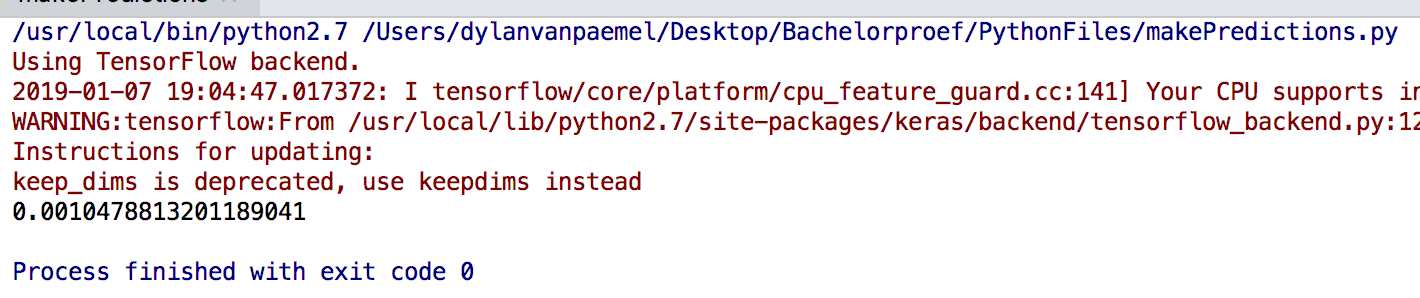
\includegraphics[width=1\textwidth]{bachproef/img/output_ml.png}
\caption{Output van de voorspelling}
\end{figure}